%%%%%%%%%%%%%%%%%%%%%%%%%%%%%%%%%%%%%%%%%%%%%%
%
%		My Thesis
%
%		EDOC Template
%		2011
%
%%%%%%%%%%%%%%%%%%%%%%%%%%%%%%%%%%%%%%%%%%%%%%


%%%%%%%%%%%%%%%%%%%%%%%%%%%%%%%%%%%%%%%%%%%%%%
%
%		Thesis Settings
%
%		EDOC Template
%		2011
%
%%%%%%%%%%%%%%%%%%%%%%%%%%%%%%%%%%%%%%%%%%%%%%
% !TEX root = ../my_thesis.tex
\documentclass[a4paper,11pt]{book}

\usepackage[T1]{fontenc}
\usepackage[utf8]{inputenc}
% % Uncomment for bibliography
% % Bibliography using Biblatex
%\usepackage{doi}
%\usepackage[autostyle]{csquotes}
% \usepackage[
%     backend=biber,
%     style=authoryear,
%     natbib=true,
%     firstinits=true,
%     sortlocale=en_US,
%     url=false, 
%     doi=true,
%     eprint=false,
%     isbn=false
% ]{biblatex}
%\addbibresource{tail/bibliography.bib}
% % OR Bibliography management for Bibtex 
% Load natbib before babel
\usepackage[round]{natbib}


\usepackage[french,german,english]{babel}


%%%%%%%%%%%%%%%%%%%%%%%%%%%%%%%%%%%%%%%%%%%%%%%
%% EDOC THESIS TEMPLATE: Variant 1.0 -> Latin modern, large text width&height
%%%%%%%%%%%%%%%%%%%%%%%%%%%%%%%%%%%%%%%%%%%%%%%
\usepackage{lmodern} % use this to fix blurry typewriter text font
%\usepackage[a4paper,top=22mm,bottom=28mm,inner=35mm,outer=25mm]{geometry}
%%%%%%%%%%%%%%%%%%%%%%%%%%%%%%%%%%%%%%%%%%%%%%%

%%%%%%%%%%%%%%%%%%%%%%%%%%%%%%%%%%%%%%%%%%%%%%
% EDOC THESIS TEMPLATE: Variant 2.0 -> Utopia, Gabarrit A (lighter pages)
%%%%%%%%%%%%%%%%%%%%%%%%%%%%%%%%%%%%%%%%%%%%%%
\usepackage{fourier} % Utopia font-typesetting including mathematical formula compatible with newer TeX-Distributions (>2010)
%\usepackage{utopia} % on older systems -> use this package instead of fourier in combination with mathdesign for better looking results
%\usepackage[adobe-utopia]{mathdesign}
\setlength{\textwidth}{146.8mm} % = 210mm - 37mm - 26.2mm
\setlength{\oddsidemargin}{11.6mm} % 37mm - 1in (from hoffset)
\setlength{\evensidemargin}{0.8mm} % = 26.2mm - 1in (from hoffset)
\setlength{\topmargin}{-2.2mm} % = 0mm -1in + 23.2mm 
\setlength{\textheight}{221.9mm} % = 297mm -29.5mm -31.6mm - 14mm (12 to accomodate footline with pagenumber)
\setlength{\headheight}{14mm}
%%%%%%%%%%%%%%%%%%%%%%%%%%%%%%%%%%%%%%%%%%%%%%


\usepackage{setspace} % increase interline spacing slightly
\setstretch{1.1}

\makeatletter
\setlength{\@fptop}{0pt}  % for aligning all floating figures/tables etc... to the top margin
\makeatother


\usepackage{graphicx,xcolor}
\graphicspath{{images/}}

\usepackage{subfig}
\usepackage{booktabs}
\usepackage{lipsum}
\usepackage{microtype}
\usepackage{url}

\usepackage{fancyhdr}
\renewcommand{\sectionmark}[1]{\markright{\thesection\ #1}}
\pagestyle{fancy}
	\fancyhf{}
	\renewcommand{\headrulewidth}{0.4pt}
	\renewcommand{\footrulewidth}{0pt}
	\fancyhead[OR]{\bfseries \nouppercase{\rightmark}}
	\fancyhead[EL]{\bfseries \nouppercase{\leftmark}}
	\fancyfoot[EL,OR]{\thepage}
\fancypagestyle{plain}{
	\fancyhf{}
	\renewcommand{\headrulewidth}{0pt}
	\renewcommand{\footrulewidth}{0pt}
	\fancyfoot[EL,OR]{\thepage}}
\fancypagestyle{addpagenumbersforpdfimports}{
	\fancyhead{}
	\renewcommand{\headrulewidth}{0pt}
	\fancyfoot{}
	\fancyfoot[RO,LE]{\thepage}
}

\usepackage{listings}
\lstset{language=[LaTeX]Tex,tabsize=4, basicstyle=\scriptsize\ttfamily, showstringspaces=false, numbers=left, numberstyle=\tiny, numbersep=10pt, breaklines=true, breakautoindent=true, breakindent=10pt}

\usepackage{hyperref}
\hypersetup{pdfborder={0 0 0},
	colorlinks=true,
	linkcolor=black,
	citecolor=black,
	urlcolor=black}
\urlstyle{same}
\ifpdf
\usepackage[final]{pdfpages}
\else
\usepackage{calc}
\usepackage{breakurl}
\usepackage[nlwarning=false]{hypdvips}
\usepackage{backref}
\renewcommand*{\backref}[1]{}
\fi
\usepackage{bookmark}

\makeatletter
\renewcommand\@pnumwidth{20pt}
\makeatother

\makeatletter
\def\cleardoublepage{\clearpage\if@twoside \ifodd\c@page\else
    \hbox{}
    \thispagestyle{empty}
    \newpage
    \if@twocolumn\hbox{}\newpage\fi\fi\fi}
\makeatother \clearpage{\pagestyle{plain}\cleardoublepage}


%%%%% CHAPTER HEADER %%%%
\usepackage{color}
\usepackage{tikz}
\usepackage[explicit]{titlesec}
\newcommand*\chapterlabel{}
%\renewcommand{\thechapter}{\Roman{chapter}}
\titleformat{\chapter}[display]  % type (section,chapter,etc...) to vary,  shape (eg display-type)
	{\normalfont\bfseries\Huge} % format of the chapter
	{\gdef\chapterlabel{\thechapter\ }}     % the label 
 	{0pt} % separation between label and chapter-title
 	  {\begin{tikzpicture}[remember picture,overlay]
    \node[yshift=-8cm] at (current page.north west)
      {\begin{tikzpicture}[remember picture, overlay]
        \draw[fill=black] (0,0) rectangle(35.5mm,15mm);
        \node[anchor=north east,yshift=-7.2cm,xshift=34mm,minimum height=30mm,inner sep=0mm] at (current page.north west)
        {\parbox[top][30mm][t]{15mm}{\raggedleft \rule{0cm}{0.6cm}\color{white}\chapterlabel}};  %the empty rule is just to get better base-line alignment
        \node[anchor=north west,yshift=-7.2cm,xshift=37mm,text width=\textwidth,minimum height=30mm,inner sep=0mm] at (current page.north west)
              {\parbox[top][30mm][t]{\textwidth}{\rule{0cm}{0.6cm}\color{black}#1}};
       \end{tikzpicture}
      };
   \end{tikzpicture}
   \gdef\chapterlabel{}
  } % code before the title body
\titlespacing*{name=\chapter,numberless}{-3.7cm}{83.2pt-\parskip}{-3.2pt+\parskip}
\titlespacing*{\chapter}{-3.7cm}{50pt-\parskip-\parskip}{30pt+\parskip+\parskip}
\titlespacing*{\section}{0pt}{13.2pt}{1em-\parskip}  % 13.2pt is line spacing for a text with 11pt font size
\titlespacing*{\subsection}{0pt}{13.2pt}{1em-\parskip}
\titlespacing*{\subsubsection}{0pt}{13.2pt}{1em-\parskip}
\titlespacing*{\paragraph}{0pt}{13.2pt}{1em-\parskip}

\newcounter{myparts}
\newcommand*\partlabel{}
\titleformat{\part}[display]  % type (section,chapter,etc...) to vary,  shape (eg display-type)
	{\normalfont\bfseries\Huge} % format of the part
	{\gdef\partlabel{\thepart\ }}     % the label 
 	{0pt} % separation between label and part-title
 	  {\ifpdf\setlength{\unitlength}{20mm}\else\setlength{\unitlength}{0mm}\fi
	  \addtocounter{myparts}{1}
	  \begin{tikzpicture}[remember picture,overlay]
    \node[anchor=north west,xshift=-65mm,yshift=-6.9cm-\value{myparts}*20mm] at (current page.north east) % for unknown reasons: 3mm missing -> 65 instead of 62
      {\begin{tikzpicture}[remember picture, overlay]
        \draw[fill=black] (0,0) rectangle(62mm,20mm);   % -\value{myparts}\unitlength
        \node[anchor=north west,yshift=-6.1cm-\value{myparts}*\unitlength,xshift=-60.5mm,minimum height=30mm,inner sep=0mm] at (current page.north east)
        {\parbox[top][30mm][t]{55mm}{\raggedright \color{white}Part \partlabel \rule{0cm}{0.6cm}}};  %the empty rule is just to get better base-line alignment
        \node[anchor=north east,yshift=-6.1cm-\value{myparts}*\unitlength,xshift=-63.5mm,text width=\textwidth,minimum height=30mm,inner sep=0mm] at (current page.north east)
              {\parbox[top][30mm][t]{\textwidth}{\raggedleft \rule{0cm}{0.6cm}\color{black}#1}};
       \end{tikzpicture}
      };
   \end{tikzpicture}
   \gdef\partlabel{}
  } % code before the title body
\titlespacing*{\part}{11.06cm}{26.4pt-\parskip-\parskip}{0pt}

\usepackage{amsmath}
\usepackage{amsfonts}
\usepackage{amssymb}
\usepackage{mathtools}
% Fix the problem with delimiter size caused by fourier and amsmath packages.
\makeatletter
\def\resetMathstrut@{%
  \setbox\z@\hbox{%
    \mathchardef\@tempa\mathcode`\(\relax
      \def\@tempb##1"##2##3{\the\textfont"##3\char"}%
      \expandafter\@tempb\meaning\@tempa \relax
  }%
  \ht\Mathstrutbox@1.2\ht\z@ \dp\Mathstrutbox@1.2\dp\z@
}
\makeatother
%%%%%%%%%%%%%%%%%%%%%%%%%%%%%%%%%%%%%%%%%%%%%%
%
%		Thesis Settings
%		Custom settings
%
%		2011
%
%%%%%%%%%%%%%%%%%%%%%%%%%%%%%%%%%%%%%%%%%%%%%%

% %
% %   Use this file for your own custom packages, command-definitions, etc...
% %
% % 
% % Packages for references - cleverref must be last
% \usepackage{nameref}
% \usepackage{hyperref}
% \usepackage{cleveref}
% \usepackage[shortlabels]{enumitem}
% % Reduce spacing in bibliography
% \setlength{\bibsep}{0pt plus 0.3ex}
% % Allow equations to break between pages
% \allowdisplaybreaks
% % Penalty for widow and orphan
% \widowpenalty=9999
% \clubpenalty=9999
% %Penalty for relation and binary operation breaks in equations
% \relpenalty=9999
% \binoppenalty=9999

\usepackage{bussproofs}
\usepackage{subcaption}
\usepackage{CJKutf8}
\usepackage{stmaryrd}
\usepackage{verbatim}
\usepackage{tikz}
\usepackage{tikz-qtree}
\usepackage{multirow}
% \usepackage{subfiles}
\setlength\heavyrulewidth{0.25ex}  % place your custom packages, etc... in this file!


%%%%%%%%%%%%%%%%%%%%%%%%%%%%%%%%%%%%%%%%%%%%%%
%%%%% HEAD: Book-Begin
%%%%%%%%%%%%%%%%%%%%%%%%%%%%%%%%%%%%%%%%%%%%%%
\begin{document}
\setlength{\parindent}{0pt}
\setlength{\parskip}{0pt} %(needs to be before titlepage and frontmatter to keep the table of contents lists short)
% \frontmatter
% \input{head/titlepage.tex}
% \include{head/dedication}
% \setcounter{page}{0}
% \include{head/acknowledgements}
% \include{head/preface}
% \include{head/abstracts}

\cleardoublepage
\pdfbookmark{\contentsname}{toc}
\tableofcontents

% % Following content is OPTIONAL (List of figures + tables)
% \cleardoublepage
% \phantomsection
% \addcontentsline{toc}{chapter}{List of Figures} % adds an entry to the table of contents
% \listoffigures
% 
% \cleardoublepage
% \phantomsection
% \addcontentsline{toc}{chapter}{List of Tables} % adds an entry to the table of contents
% \listoftables
% your list of symbols here, if needed.


% space before each new paragraph according to the template guidelines.
%(needs to be after titlepage and frontmatter to keep the table of contents lists short)
\setlength{\parskip}{1em}


%%%%%%%%%%%%%%%%%%%%%%%%%%%%%%%%%%%%%%%%%%%%%%
%%%%% MAIN: The chapters of the thesis
%%%%%%%%%%%%%%%%%%%%%%%%%%%%%%%%%%%%%%%%%%%%%%
\mainmatter

\cleardoublepage
\part{Background}
\chapter{The phenomenon of structural repetition}
    
    \graphicspath{{main/chapter1/Intro: structural repeat/figs/}}
\section{Defining repeat}
\begin{comment}
Section goal: Motivate the notion of structural repeat
- [requirement 1] This section should be readable for general audience. All examples should be simple, intuitive, and common. 
- [requirement 2] This section should fully establish why defining repeat as a cognitive phenomenon is nontrivial. 
- [requirement 3] This section should build up the concept (structural repeats) incrementally, starting from the simplest notion of repeat. Each increment of the concept should highlight the part that is new and explain what additional explanation power it gives. 
- [requirement 4] This section should only introduce the formal notations only after the reader has understood the nuances of the concept intuitively and verbally. 

Plan: 
    - intro
    - First approximation: Equality of the observations 
        - Can explain: 
        - Can't explain: Postman example of ``doing the same thing''
        - Limitation: we sometimes also experience non-exact repeat
        - Core problem: (Categorization) An entity is characterized by its external properties and affordance.  
    - Second approximation: Equality of the Abstraction 
        - e.g. conceptual category, intention, particular features, internal relations
        Equality of the generative program underlying the observation. (the instantiation of a abstract concept can be subsumed as a generative program)
        - Invariance? 
        - Can't distinguish: parralel syntax 
    - Third approximation: Equality of the Interpretation 

    - Structural repeat




    
    Extensional vs Intentional equality
    - Third approximation: Intentional equality of the generative programs underlying the observation
    https://oecs.mit.edu/pub/vgigt1aq/release/1?from=10215&to=11248
    https://oecs.mit.edu/pub/vgigt1aq/release/1?from=12735&to=13964
\end{comment}

% The central topic of this thesis is about the computational modeling of repetitions in music in a cognitively plausible way. 
% Although repetition in music might be different from other domains, we first focus on the aspects that is generally applicable in other domains. 
% Repetition is a core feature of our musical experience. Since music is fundamentally a mental phenomenon, perhaps it is helpful to first take a birds-eye-view on how human we experience repetition in general.

We experience repetition in diverse domains: we discern shared narrative structures across novels, films, and music, and we uncover universal laws governing phenomena as distinct as ocean currents and atmospheric dynamics. Moreover, humans can abstract patterns of patterns, as seen in the application of category theory to mathematics and programming. These examples illustrate our remarkable ability to not only detect abstract repetitions but also to productively employ them in navigating both the physical and mental worlds.

Repeat, as we intuitively perceive it, is surprisingly nontrivial to formalize. 

\subsection{Repeated observations}
Let us first approximate our experience of repeat with a simple characterization: \textbf{a specific observation occurs across time and space}. We can find examples across domains that fit this definition. For instance, an ongoing fire siren corresponds to a repeat of a specific sound across time. The decorative motifs found in mosaic tiling are repeats of a visual symbol across space. The periodic motion of a pendulum contains repeats of a specific movement. To put it formally: 

\begin{equation} 
    \tag{Approximation 1}
    \llbracket x_2 \ \emph{repeats}\  x_1  \rrbracket\footnote{We adopt the notation $\llbracket \dots \rrbracket$ from formal semantics as a function that maps a expression to its truth condition}  =\left\{ x_2 = x_1\right\}
\end{equation}

Our first definition is simple and precise, and its mental processing of can be computationally modelled in a straight forward manner. However, it does not fully capture of our \emph{intuitive experience} of repeat. Consider a postman, when frustrated by his mundane work, complains about ``doing the same thing'' over and over again. Clearly, by ``doing the same thing,'' our imaginary postman does not mean it as repeating a list of concrete physical actions (e.g., turning right on the crossroad at 7:23 am, and stopping his car at the exact same spot). If the postman's job can be just explained as such, imagine the catastrophes caused by a mail robot programmed to do exactly that. 

In order to make the postman's expression work, our model of repeat should allow some degrees of flexibility. For example, there are multiple ways to achieve the same task of ``parking the car'' depending on the situation at hand. What if the closest parking slot is occupied? What if there are kids walking by? What if there are construction works blocking the entire side of the street? "Just do the sensible things" would be a typical response from human. In those scenarios, the observed actions would be adapted to include extra stepping on gas and break, checking the mirrors/traffic lights/pedestrians, looking for available parking slots. Then to our robot friend, in what ground can it understand these "sensible adaptions" of actions as being the ``same''? 

One might try to incorporate this kind of non-exact repeat by proposing some kind of function that measure the similarity/dissimilarity among the instances. For example, one might say if two list of actions both ends with stopping the car and getting out the car, we define a high similarity among them. But there are cases where our experience of repeat is not about the similarity of the observations at all. Consider a cityscape of New York where we find repetitions of buildings. Each building can be very different from the image perspective. 
% If we go back to visual patterns, we find variations also across instances of repeats. So our "ill-defined" notion of repeat also fails there. So the problem of our definition is just limited to one domain but is a general issue.
% For visual case, one can potentially measure the pixel-wise L2 distance (MSE). 

The reason we perceive repeat is that we interpret these visuals as concrete instances of the same abstract concept: building, which we know which properties and functions they should have. Thus, the core problem of the first definition is that it describes the phenomenon of the perceived repeat purely as a property of the observations themselves, without involving a mental model that explains and thus predict the observations. This problem can not be fixed without incorporating the mental understanding of the observations in our formulation of repeat.  

\subsection{Repeated abstractions}

If we think of the ``mental understanding'' as the ability to associate a specific token with its category/type, our next approximation of repeat would be ``instantiations of the same category/type''. 
\begin{equation} 
    \tag{equal abstraction}
    \llbracket x_2 \ \emph{repeats}\  x_1  \rrbracket = \left\{ \text{Type}(x_1) = \text{Type}(x_2)\right\}
\end{equation}

By shifting the focus from observations to their abstractions, we can explain the postman's notion of ``doing the same thing'' as multiple instantiations of abstract action ``parking the car'' or ``inserting mail to mailboxes'' on different situation-encoding parameters such as ``the location of the next closest parking slot'' and ``whether there are objects blocking the path''. In the case of New York's cityscape, each appearance of the buildings can be thought of as an instantiated token from the type ``building'' using different configurations such as the building's height, style, year, and the angle facing the viewer, etc. 

Despite the generality of the approach, it may sometimes ignore too much information for our experience of repeat. Take the following exerpt from a Chinese poem for example, despite the different in the concrete words, we see a clear parallelism (as a form of repeat) in the two phrases. Is it the abstraction that is repeated? Technically yes, since each of the two phrases can be understood syntactically as a noun phrase. But something very important is missing if we simply say these two phrases contains repeat just because they are both noun phrases. If we substitute the second phrase with any other noun phrase, our previous experience of parallelism imediatelly disappear. One can notice that their are some correpondence between the structure of this two phrases. In term of grouping, ``[bright] [moon]'' correponds to ``[clear] [spring]'' and ``[pine] [among] [shine]'' correponds to ``[stone] [on] [flow]''. Not only each of the corresponding character are from same syntactic category, the syntactic structures of the two phrases are identitcal as demonstrated in Figure \ref{fig: Chinese poem}. Furthermore, the meaning of the correponding words all aims to convey a feeling of serenity.  
\begin{figure}
    \centering 
    
\includegraphics[width=0.8\linewidth]{chinese peom surface}
    \caption{Exerpts from the poem () written by Wang Wei (699–761 during Tang dynasty), translated by Xu Yuanchong}
    % %Such kind of parallel is not an incident but almost a requirement in Tang poetry, which support human's ability the both recognize and generalize such patterns.}
    \label{fig: Chinese poem surface}
\end{figure}

\subsection{Repeated interpretations}

% Perhaps a more general way to expressive our experience of repeat is \textbf{the reoccurrence of some invariance of interest underlying the observations}. 





% A natural next step of our approximation is: \textbf{outputs of the same program on given different inputs}. Here an important distinction is made: we test the equality of the programs instead of equality of their outputs. With this modification of our approximation, we can explain the postman's notion of ``doing the same thing'' as calling the same functions ``parking the car'' or ``inserting mail to mailboxes'' on different situation-encoding parameters such as ``the location of the next closest parking slot'' and ``whether there are objects blocking the path''. The output of these functions results in concrete actions, which are different on the face value. More precisely, if we have two observations $y_1$ and $y_2$, we say they are repeated if there exist a function $f$ and input parameters $x_1$ and $x_2$ such that $y_1 = f(x_1), y_2 = f(x_2)$.


% \begin{equation} 
%     \tag{Approximation 2}
%     \llbracket y_2 \ \emph{repeats}\  y_1  \rrbracket = \left\{ \exists f\ x_1\ x_2,\quad  f(x_1)=y_1 \wedge  f(x_2) = y_2\right\}
% \end{equation}



\subsection{Repetition within a structure}



So far we have only concerned repetition as a \emph{perceived} property of observations. 



\begin{equation} 
    \tag{Approximation 3}
    \llbracket y_2 \ \emph{repeats}\  y_1  \rrbracket = \left\{ \exists R\ x_1' \ x_2' \ x_1\ x_2,\quad  x_1' R x_1 \wedge   x_2' R x_2 \right\}
\end{equation}


% One way to model such flexibility is to see these concrete instances of repeats as \textbf{outputs of the same program (model/function) but given different parameters}. This characterization is fairly simple to model computationally in the generative direction (e.g. as in procedurally generated visual scene), but is much harder the implement in the direction of perception.

% \begin{equation} 
%     \tag{}
%     \llbracket y_2 \ \emph{repeats}\  y_1  \rrbracket = \left\{ 
%         y_1=g(f_1(x_1)) \wedge y_2 = g(f_2(x_2))
%     \right\}
% \end{equation}


% \begin{table}
%     \centering
%     \begin{tabular}{p{0.3\linewidth}  c  c}
%         Approximations & Examples & Required mechanisms \\
%         \toprule
%         The same concrete observation occurs in different time and space.  & e & d\\
%         \hline
%         The same model being instantiated with different parameters. & df &\\
%         \hline
%         The same relation instantiated with different abstractions of observations. & df &
%     \end{tabular}
%     \caption{}
% \end{table}

% \begin{table}
%     \centering
%     \begin{tabular}{l l l}
%         Notion of equality & non-structural & structural \\
%         \toprule
%         Exact  & $\exists f g x_1 x_2, f(x_1) = g(x_2) \wedge f \simeq g$  & $\exists f g x_1 x_2, f(x_1) = g(x_2) \wedge f \equiv g$ 
%         % \hline
%         % Non-exact & $\exists f_1 f_2 g_1 g_2 x_1 x_2, f_1(f_2(x_1)) = g_1(g_2(x_2)) \wedge f_1 \simeq g_1$  & $\exists f_1 f_2 g_1 g_2 x_1 x_2, f_1(f_2(x_1)) = g_1(g_2(x_2)) \wedge f_1 \equiv g_1$ 

%     \end{tabular}
%     \caption{}
% \end{table}

% \begin{table}
%     \centering
%     \begin{tabular}{l p{0.3\linewidth} p{0.3\linewidth}}
%         $f$, $g$ share the same & upper-level & lower-level  \\
%         \toprule
%         formalization  & $\exists f_1 f_2 g_1 g_2, f = f_1 \circ f_2\wedge g = g_1 \circ g_2 \wedge f_1 \equiv g_1$  & $\exists f_1 f_2 g_1 g_2, f = f_1 \circ f_2\wedge g = g_1 \circ g_2 \wedge f_2 \equiv g_2$\\
%         \hline
%         examples & variations of K331 (same upper level reduction with different lower level realization) & bach C major prelude (same figuration across phrases with different harmony reduction)
%         % Non-exact & $\exists f_1 f_2 g_1 g_2 x_1 x_2, f_1(f_2(x_1)) = g_1(g_2(x_2)) \wedge f_1 \simeq g_1$  & $\exists f_1 f_2 g_1 g_2 x_1 x_2, f_1(f_2(x_1)) = g_1(g_2(x_2)) \wedge f_1 \equiv g_1$ 
%     \end{tabular}
%     \caption{}
% \end{table}

% \begin{table}
%     \centering
%     \begin{tabular}{p{0.4\linewidth}  p{0.4\linewidth}}
%         Object & Domain \\
%         \toprule
%         {\begin{itemize}
%             \item Concrete observation
%             \item Generative program 
%             \item Relation
%         \end{itemize}} 
%         & 
%         {\begin{itemize}
%             \item Time
%             \item Space
%             \item Levels of abstraction 
%         \end{itemize}}
%         % {\begin{itemize} \item Time \item Space \item Levels of abstraction \end{itemize}}\\

%     \end{tabular}
%     \caption{}
% \end{table}


% \paragraph{Attempt 1: The same concrete observation occurs in different time and space.}

% Required computational mechanisms : 
%     - production: duplication 
%     - understanding: equality testing
% Failed reason: too little flexibility, does not take abstractions into account.

% \paragraph{Attempt 2: The same pattern being instantiated in different time and space.}

% Required Computational mechanisms (given the space of generative function) (on top of attempt 1): 
%     - production: sampling function parameters, function application
%     - understanding: 

% \paragraph{Attempt 3: The same groups of relation governing abstractions of observations.}




% \end{document}

\section{Structural Repeat}
Our experience of repeat can be evalated by structure. In an informal way, we mean ``structure'' as ``how things are put together'' or equivalently, ``how things can be elaborated''. In language, the syntactic structure describes how words can combine to form a correct sentence, the semantic structures describes how meanings can combine to form new meanings. In action planning, structure describes how actions and goals can be broken into smaller components. In music, tonal structure describes how voices and harmony can be prolonged (elaborated through time). 

\subsection{Example 1: Chinese Poetry}
Parallel syntax is the phenomenon when two phrases have the identical syntactic structure. An example is shown in Figure \ref{fig: Chinese poem}. This kind of repeat is hardly a happy coincidence. It is often the case that the semantic meanings also forms either synonyms or contrast. 
\begin{figure}
    \centering 
    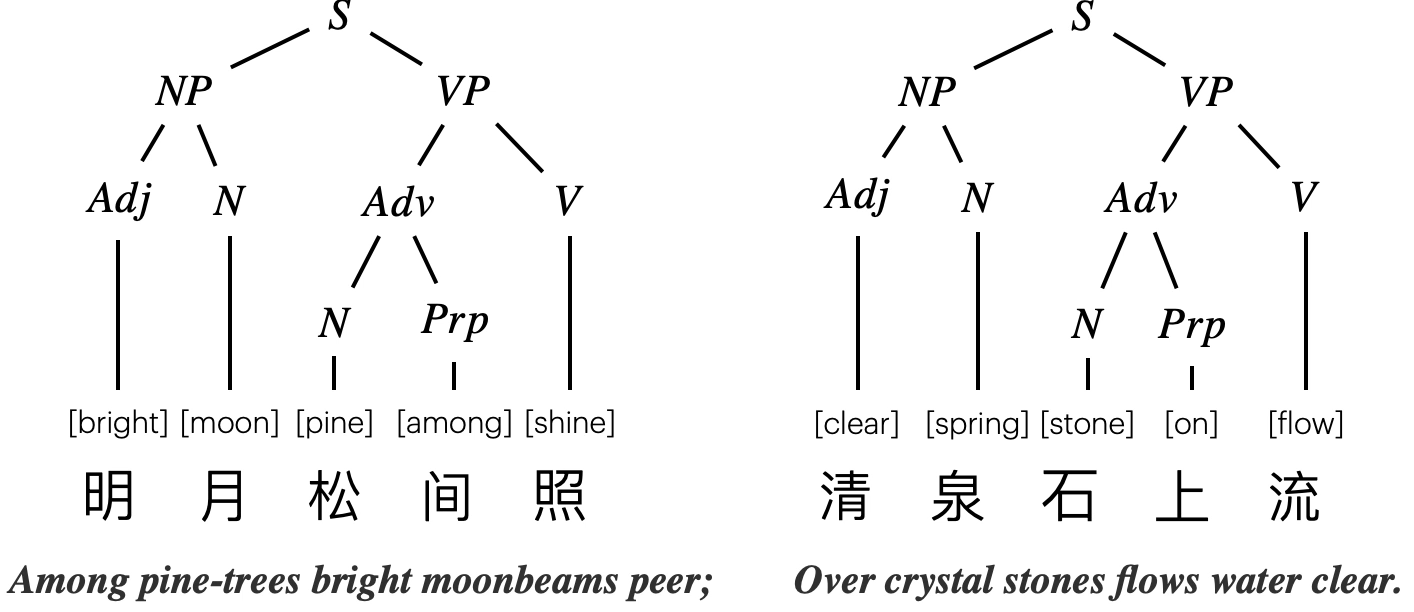
\includegraphics[width=0.8\linewidth]{Chinese poem.png}
    \caption{A poetry written by Wang Wei (699–761 during Tang dynasty), translated by Xu Yuanchong, exhibiting parallel syntactic structure.} 
    % %Such kind of parallel is not an incident but almost a requirement in Tang poetry, which support human's ability the both recognize and generalize such patterns.}
    \label{fig: Chinese poem}
\end{figure}

\subsection{Example 2: Making coffee}
Imagine John performed the following list of actions: he measures 18 grams of coffee ground, put these measured coffee ground into a coffee maker, he then measures 150 ml of water, and put the measured water into the coffee maker, then he activates the coffee machine. 

% We can perceive the repetition of this composite actions "measuring x amount of y and put y into the coffee maker". 

The ``structure'' in this example is about the meaning of these actions: what does each action achieve and how does these list of actions accomplish a single goal? (How actions are put together). 
We analyze this scenario by interpreting an action as a particular way to achieve a goal. To make things simple, goals are interpreted as changes in the state of the world. For example, the overarching goal in this example is that John want to transform his state from "having coffee bean and water supply" into ``having a cup of coffee''. 

Goals can be combined in two general and natural ways, the first is sequential composition (chaining): if we know how to accomplish $x\to z$ and $z\to y$ we can accomplish the goal $x \to y$ by concatenating the two actions (also feeding the result of the action to the next action). The second is parallel composition, if we can accomplish $x_1 \to y_1$ and $x_2 \to y_2$, we can also accomplish $(x_1,x_2) \to (y_1,y_2)$. The tuple notation denotes the conjunction of states. 

\begin{figure}
    \centering 
    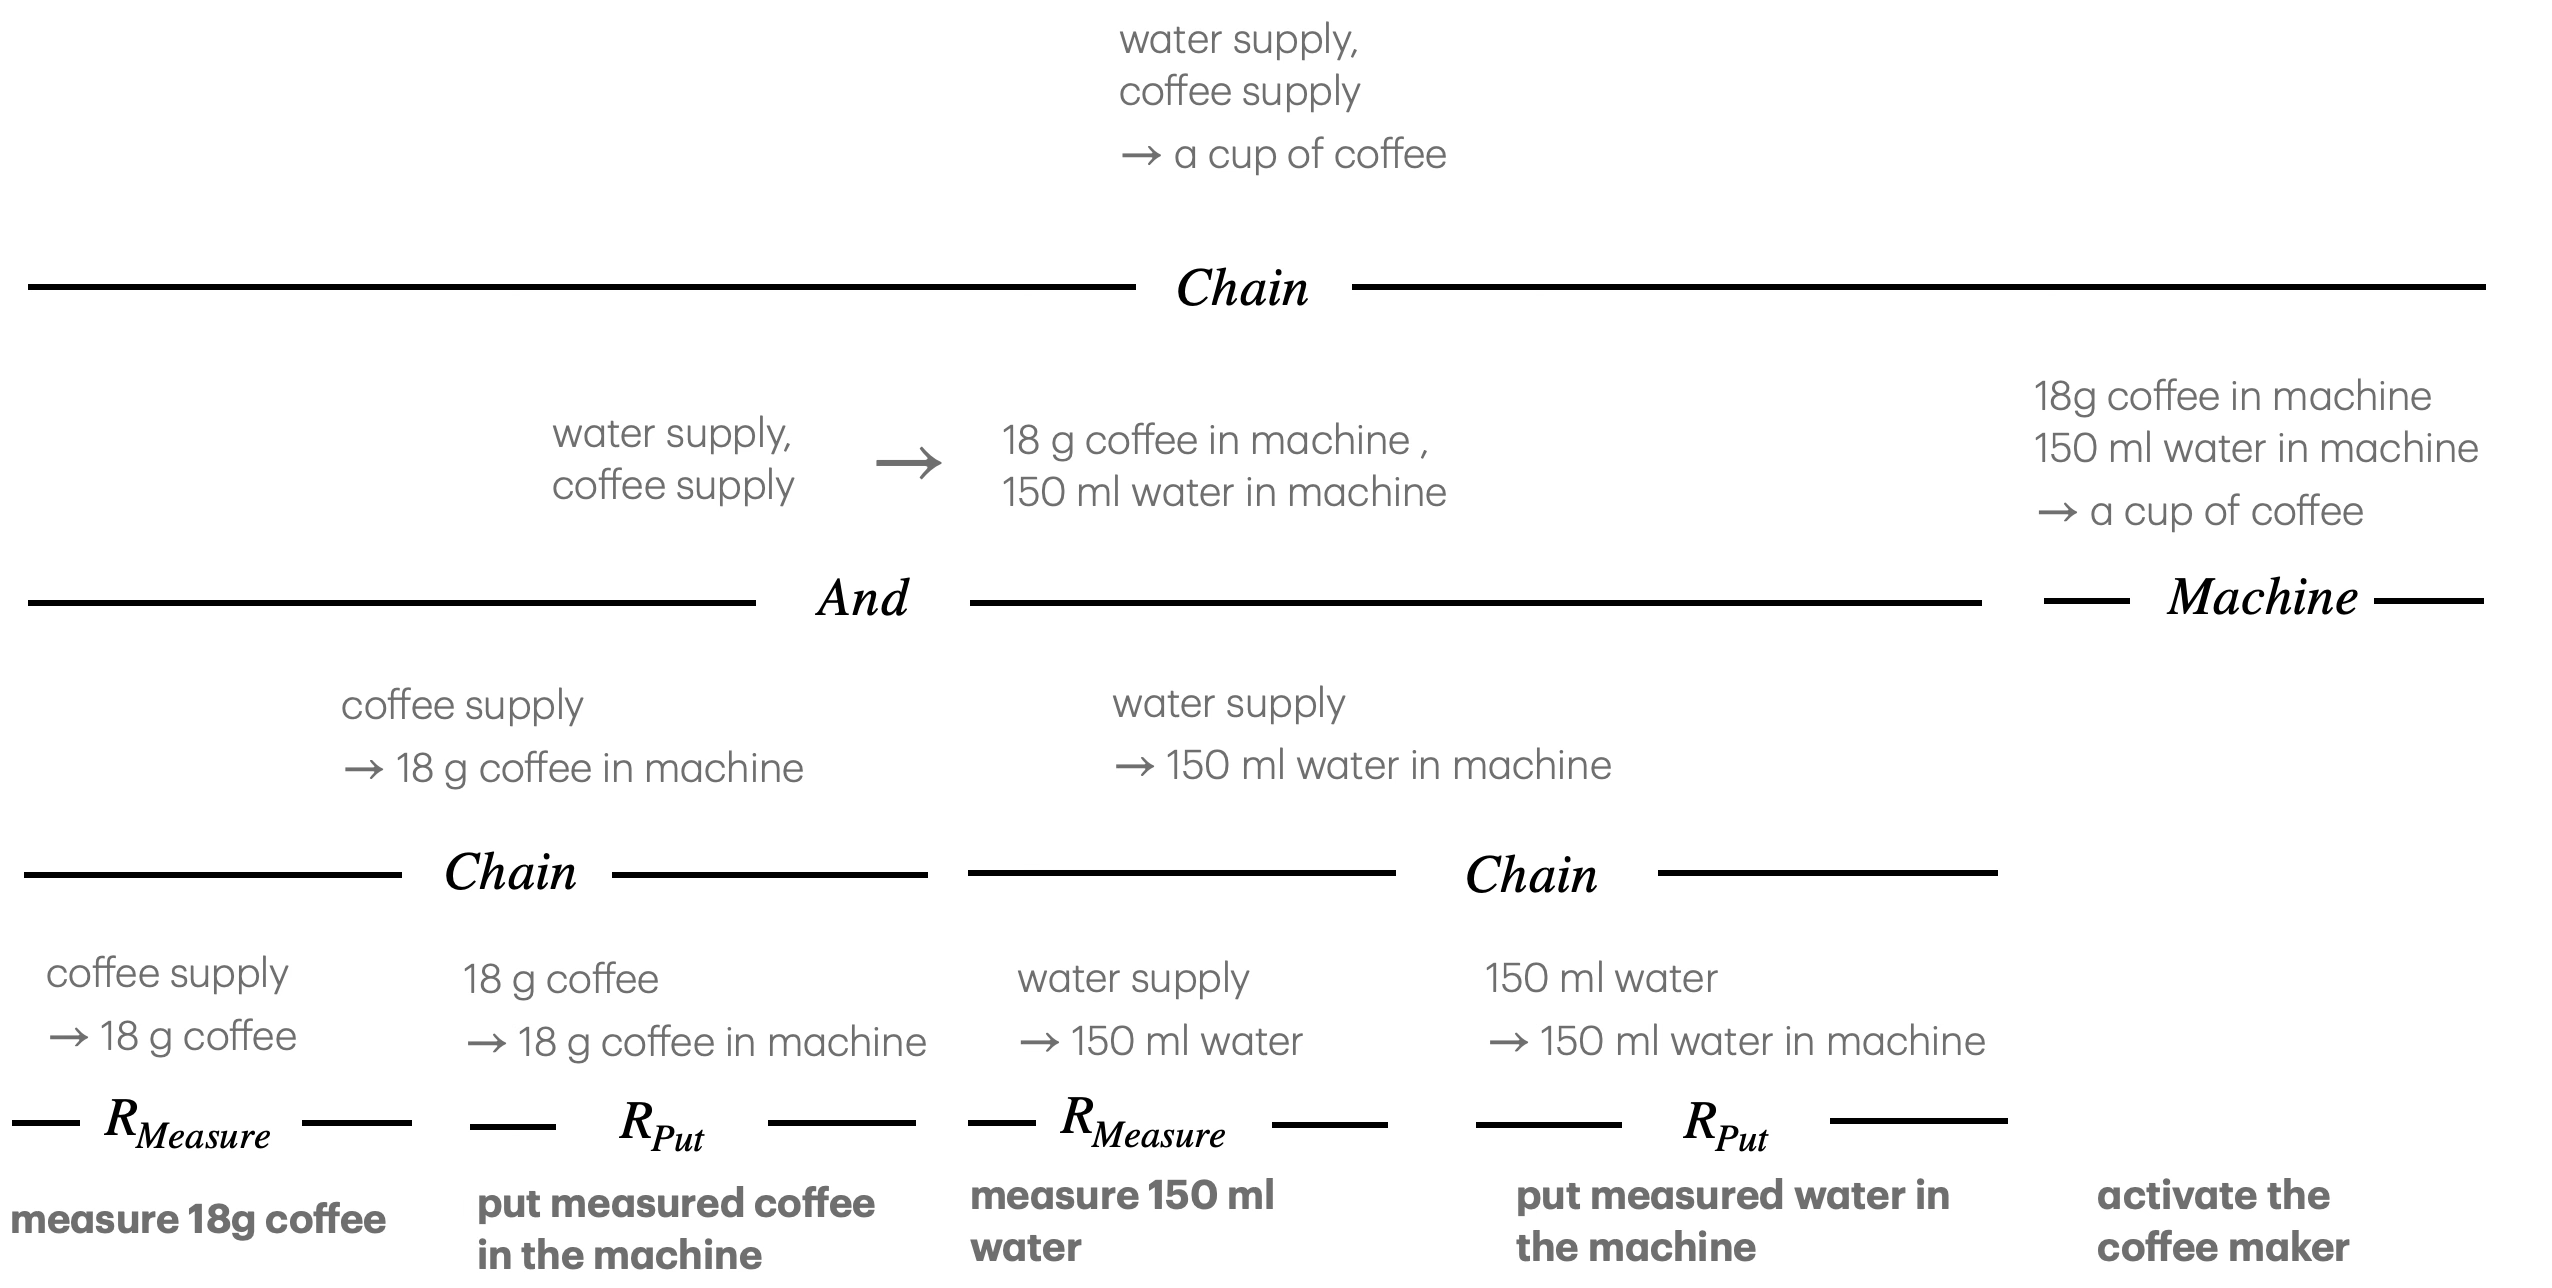
\includegraphics[width=0.9\linewidth]{coffee.png}
    \caption{}
    \label{fig: coffee}
\end{figure}

\begin{figure}
    \centering 
    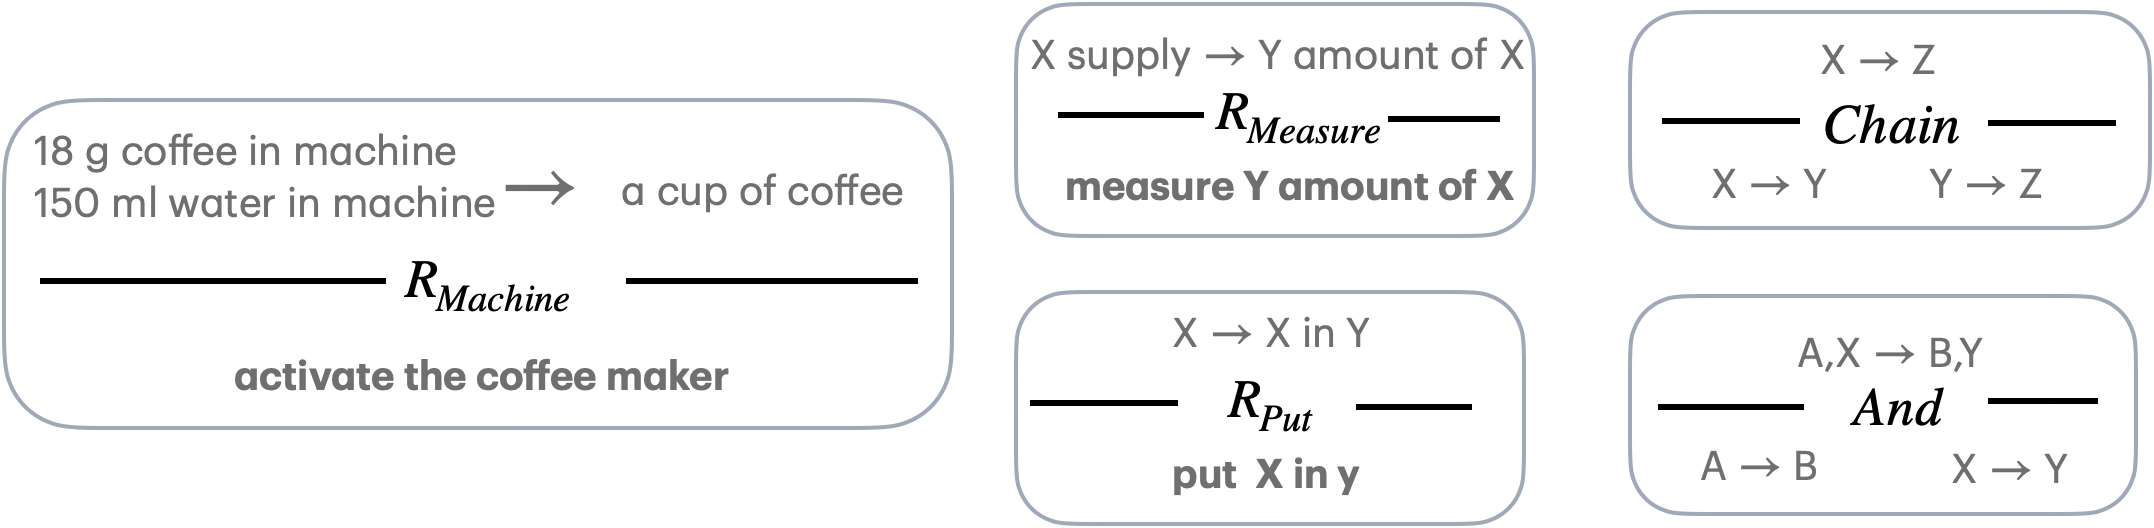
\includegraphics[width=0.9\linewidth]{coffee rule.png}
    \caption{}
    \label{fig: coffee rule}
\end{figure}

The action of measuring 18 grams of coffee bean is a solution of the goal  ``having a bag of coffee bean \to having 18 grams of coffee bean''

The action of put 



        % \subsection{Making coffee} 
        %     % \import{main/chapter1}{Making coffee}{Making coffee}
        % \subsection{Comics}
        % \subsection{Classical Chinese poem}
    \section{Cognitive principles underlying syntactic repetition}
        \subsection{Compossibility}
        \subsection{Efficient reuse of computations}
        \subsection{Minimizing description length}


\chapter{Syntactic repetition in tonal music}
    \section{Hierarchical structure in Music}
        \subsection{Form, rhythm, harmony}
    \section{Repetition in Music}
        \subsection{Exact vs varied}
        \subsection{Syntactic vs non-syntactic}
        \subsection{Differentiating reuse and repeat}


\chapter{Bayesian model-based reasoning}
    \section{Generative models}
    \section{Functional Probabilistic Programming}
        \subsection{Markov category and probability monads}
        \subsection{Synthetic probability theory and Quasi-Borel space}
        \subsection{Bayesian non-parametrics}




%\include{main/ch2_figures_tables}
\cleardoublepage
\part{Template Grammar}
% \chapter{Deriving template grammar from first principles}
    \section{Abstraction of composition}



        \subsection{Tree-substitution grammar}
    \section{Abstraction of repetition}
        What is a computational process that allow us from understanding 
        "catcat", "1414", "$\triangle\triangle$" as instantiations of same pattern $x \mapsto (x,x)$?

        Notice that these three examples are different in both their token types 
        and the length of the repeating unit.

        \subsection{Pattern language}
    \section{Abstraction of composition with repeat}
        \subsection{Repetition combinators}

        Let $f : A \to B, g: X \to Y$ their tensor product is defined as
        \begin{align*}
            f \otimes g : A \times X  &\to B \times Y\\
            (f \otimes g)(a,x) &= (b,y)
        \end{align*}
        It is further required that this tensor product is associative, i.e. $(f \circ g) \circ h \simeq f \circ (g \circ h)$.

        $$
        (g, (f_1,...,f_n)) \mapsto g \circ (m_g(f_1,...,f_n))
        $$
        where $m_g$ is a function that duplicates its $n$ inputs into $k$ outputs where $n\leq k$.  
        $$
        m_g (f_1,...,f_n)= g\circ \bigotimes_{i=1}^k f'_i  \quad \text{where} \quad 
        f'_i \in \{g,f_1,...,f_n\}
        $$
        The set of all such functions can be defined constructively
        

        \subsection{Introducing template grammar}
            \begin{align}
                \mathbb S &:= \_\_ \ | \ \star \ |\  \mathbb N^+ \\
                \mathbb M &:= \mathbb S ^ *\\
                \mathcal T &:= E \ |\  (\mathbb N, \mathcal T, \mathcal T) \ |\  (\mathcal T, \mathbb M, \mathcal T^*)
            \end{align}

            
            

        \subsection{Template grammar as a probabilistic program}
        
\pgfmathsetmacro {\vizWidth}{0.24}
\chapter{Parsing of Template grammar}
    \section{Parsing as weighted deduction} 
    \section{A polynomial time semi-ring parsing algorithm}
    \subsection{Notations}
        Like a production rule, a template $\alpha \in \mathcal T$ may expand a non-terminal $X \in NT$ into 
        a list of symbols. The resulted $n$ non-terminals divides the terminals into $n+1$ chunks.
        We call these chunks as the \emph{evidence} of $\alpha$ on $X$. 
        We denote this ternary relations among 
        a head non-terminal $X$, a template $X$, and an evidence $e$ as $X \xrightarrow{\alpha} e$
        
        The goal of parsing template grammar is to understand how 
        a list of list of terminals, as the evidence for some template on the start symbol $S$. 
        \subsubsection{Item form:} 
            Each item is a triple $(NT, \mathcal{T},{T^*}^*)$ denoted as 
            \begin{equation} {X \xrightarrow{\alpha} e}
            \end{equation}
            which corresponds to the proposition "the evidence resulted from 
            template $\alpha$ on the non-terminal $X$ is $e$"
        
        

         
        \subsubsection{Inference rules}

        % \setlength{\tabcolsep}{15pt}
        % \renewcommand{\arraystretch}{1}
        \begin{tabular}{l c c}

            \midrule\\
            \textbf{Zero-hole}\\
            
            $\textsc{Complete}^{\langle \_ \rangle}_0$  &
            \begin{minipage}{\vizWidth\textwidth}
                \medskip
                {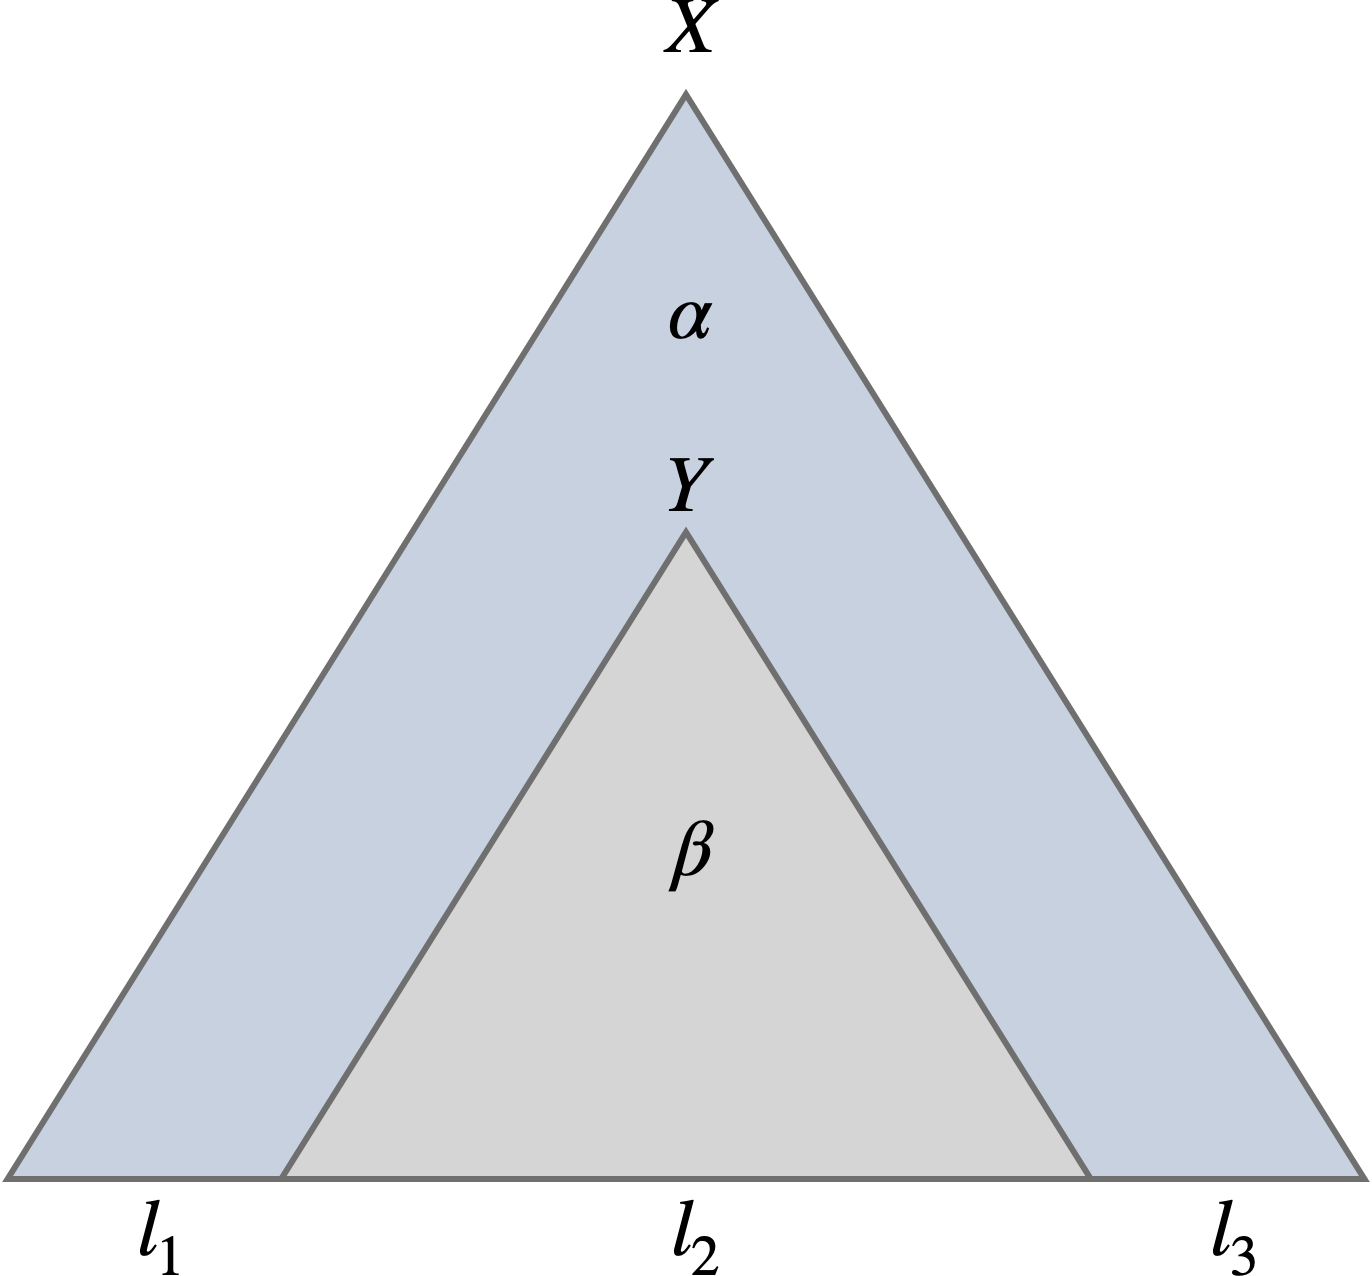
\includegraphics[width=\linewidth]{images/parsing/complete[New][0].png}}
            \end{minipage} &
            \AxiomC{$X \xrightarrow{\alpha} [l_1,l_3]$}
            \AxiomC{$Y \xrightarrow{\beta} [l_2]$}
            \RightLabel{$\substack {l_2 \neq [\ ] \\ X \overset{\alpha}{\leadsto}  [Y]}$}
            \BinaryInfC{$X \xrightarrow {(\alpha,\langle \_\rangle, [\beta])} {[l_1+l_2+l_3]}$}
            \DisplayProof\\
            
           
            $\textsc{Complete}^{\langle \_ \  \_ \rangle}_{0,0}$ &
            \begin{minipage}{\vizWidth\textwidth}
                \medskip
                {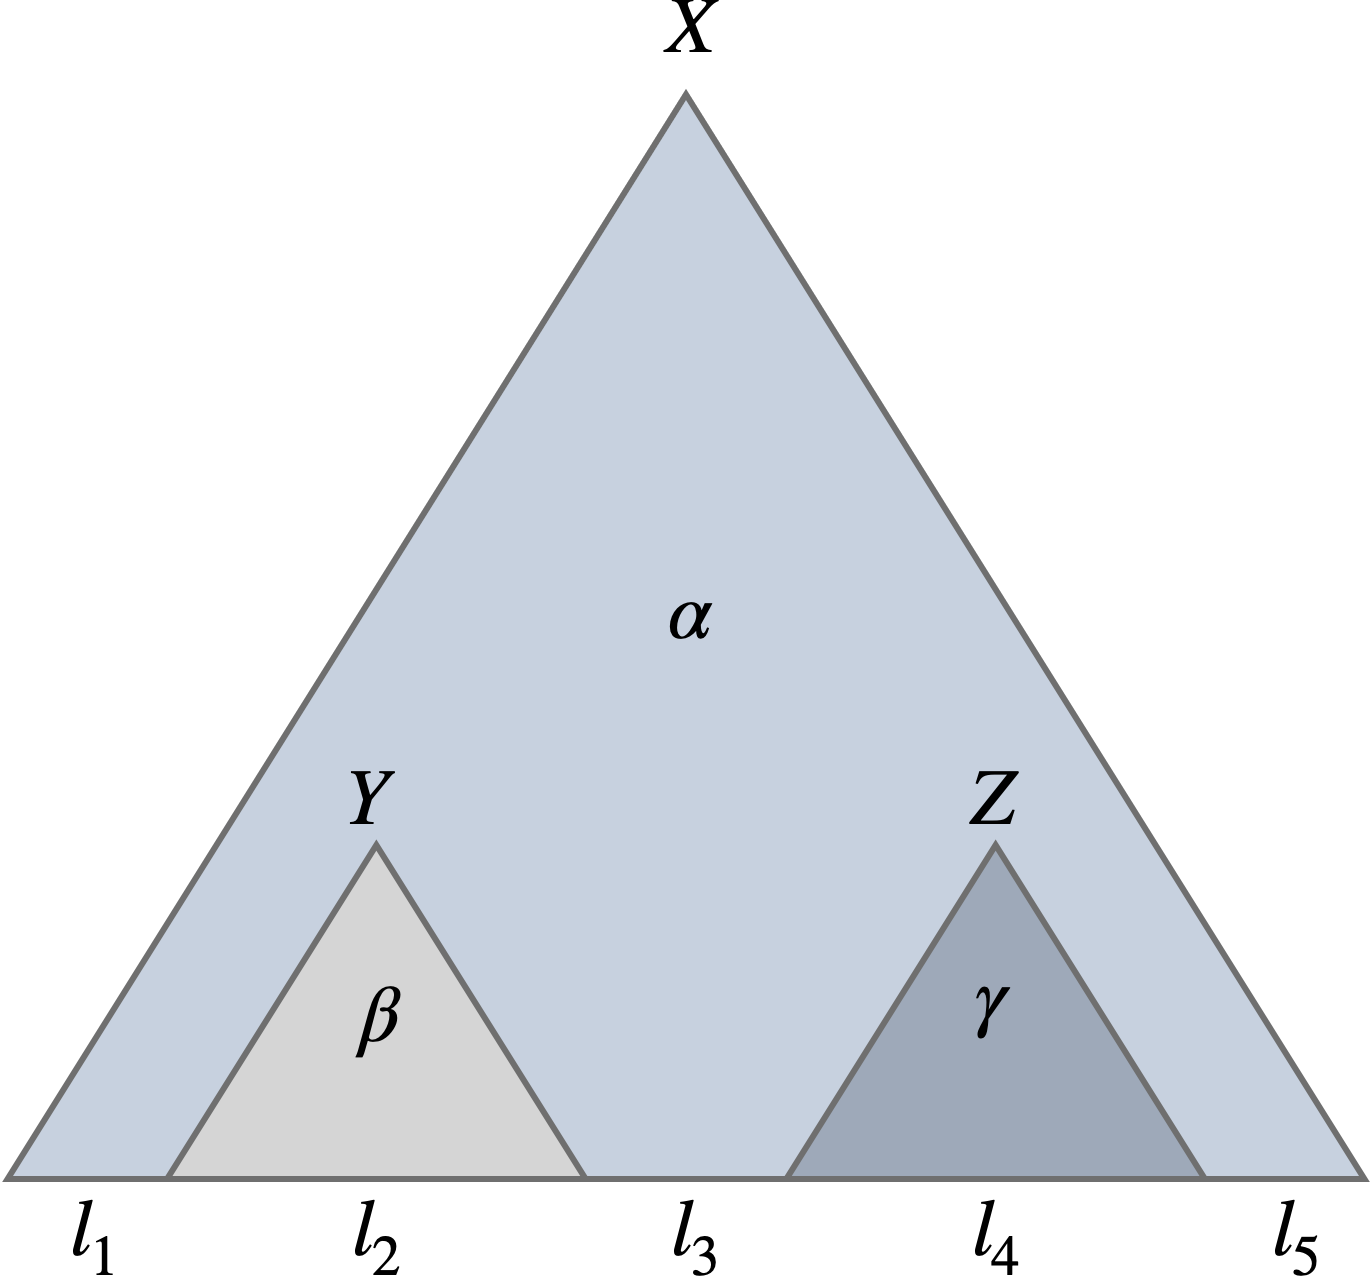
\includegraphics[width=\linewidth]{images/parsing/complete[New,New][0,0].png}}
            \end{minipage} &
            \AxiomC{$X \xrightarrow{\alpha} [l_1,l_3,l_5] $}
            \AxiomC{$Y \xrightarrow{\beta} [l_4]$}
            \AxiomC{$Z \xrightarrow{\gamma} [l_4]$}
            \RightLabel{$\substack{l_2,l_4 \neq [\ ] \\ X \overset{\alpha}{\leadsto} [Y,Z]}$}
            \TrinaryInfC{$X \xrightarrow {(\alpha,\langle \_ \ \_ \rangle, [\beta, \gamma])} {[l_1+l_2+l_3+l_4+l_5]}$}
            \DisplayProof\\
            
            
            $\textsc{Complete}^{\langle \_ \  1 \rangle}_{0,0}$ &
            \begin{minipage}{\vizWidth\textwidth}
                \medskip
                {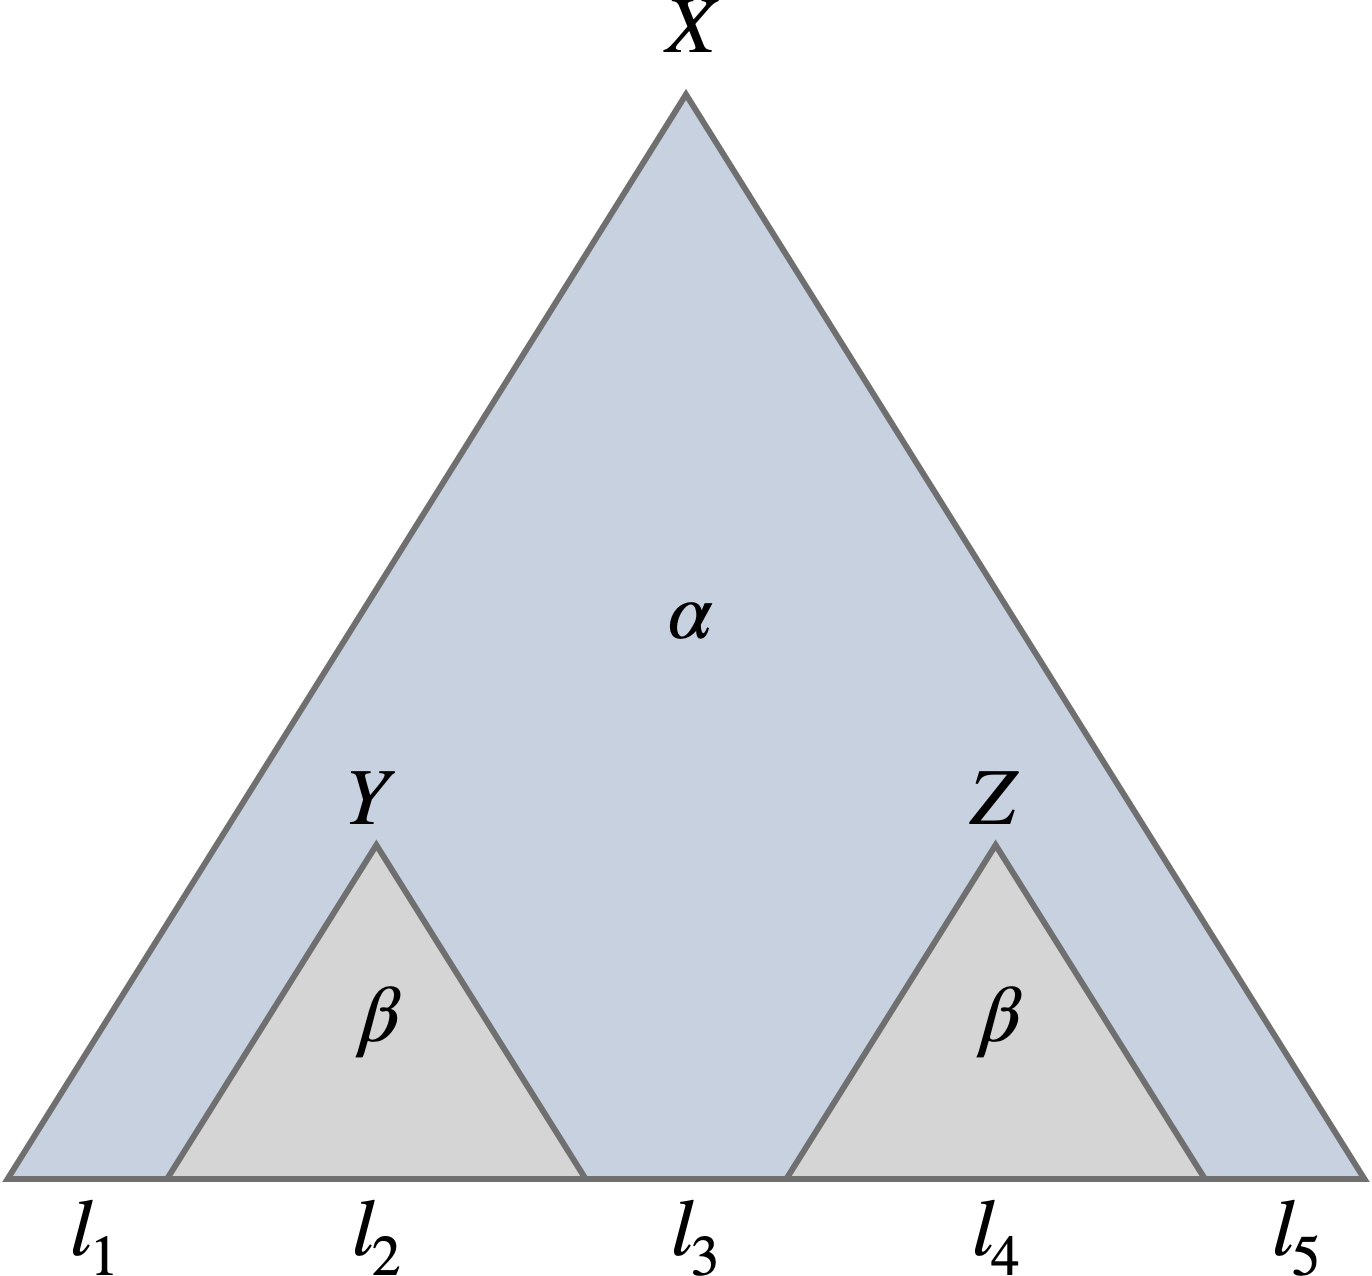
\includegraphics[width=\linewidth]{images/parsing/complete[New,1][0,0].png}}
            \end{minipage} &
            \AxiomC{$X \xrightarrow{\alpha} [l_1,l_3,l_5] $}
            \AxiomC{$Y \xrightarrow{\beta} [l_4]$}
            \AxiomC{$Z \xrightarrow{\beta} [l_4]$}
            \RightLabel{$\substack{l_2,l_4 \neq [\ ] \\ X \overset{\alpha}{\leadsto} [Y,Z]}$}
            \TrinaryInfC{$X \xrightarrow {(\alpha,\langle \_ 1 \rangle, [\beta])} {[l_1+l_2+l_3+l_4+l_5]}$}
            \DisplayProof
        \end{tabular}
        
        
        \begin{tabular}{l c l}
            \midrule\\
            \textbf{One-hole}\\

            $\textsc{Complete}^{\langle \star \rangle}_1$ &
            \begin{minipage}{\vizWidth\textwidth}
                \smallskip
                {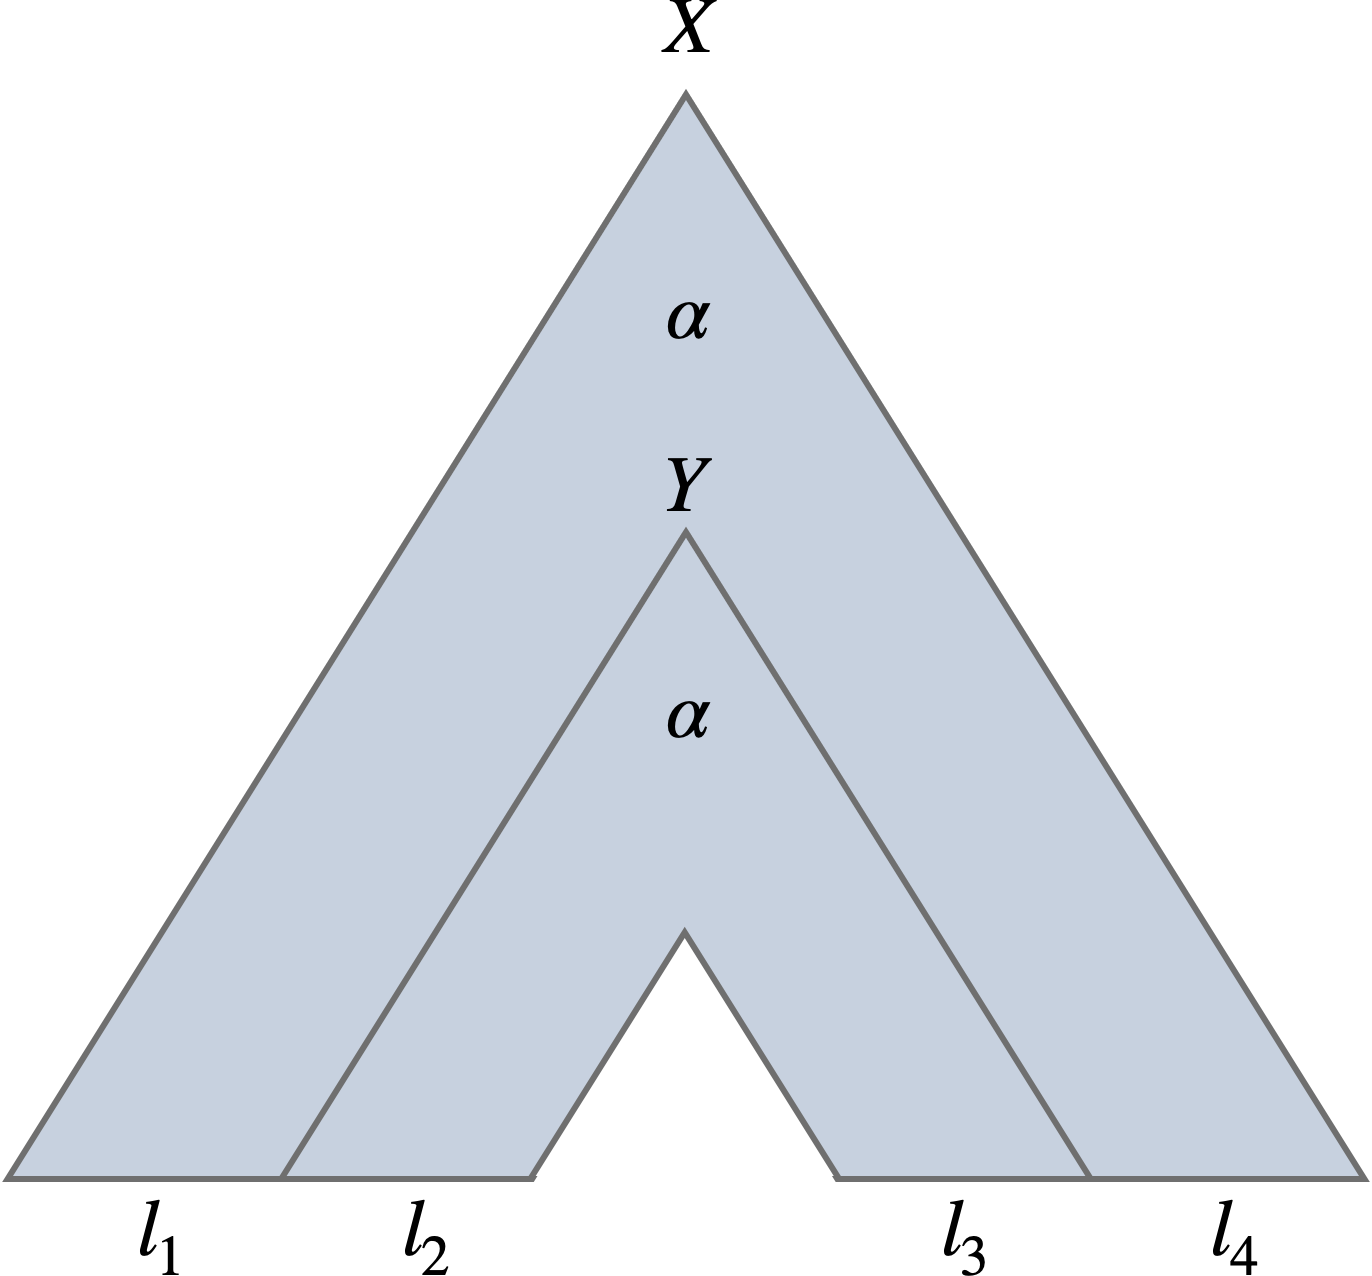
\includegraphics[width=\linewidth]{images/parsing/complete[Star][1].png}}
            \end{minipage} &
            \AxiomC{$X \xrightarrow{\alpha} [l_1,l_4] $}
            \AxiomC{$Y \xrightarrow{\alpha} [l_2,l_3]$}
            \RightLabel{$\substack {X \overset{\alpha}{\leadsto} [Y]}$}
            \BinaryInfC{$X \xrightarrow {(\alpha,\langle \star \rangle, [\ ])} {[l_1+l_2,l_3+l_4]}$}
            \DisplayProof\\
        
            $\textsc{Complete}^{\langle \_ \rangle}_1$ &
            \begin{minipage}{\vizWidth\textwidth}
                \smallskip
                {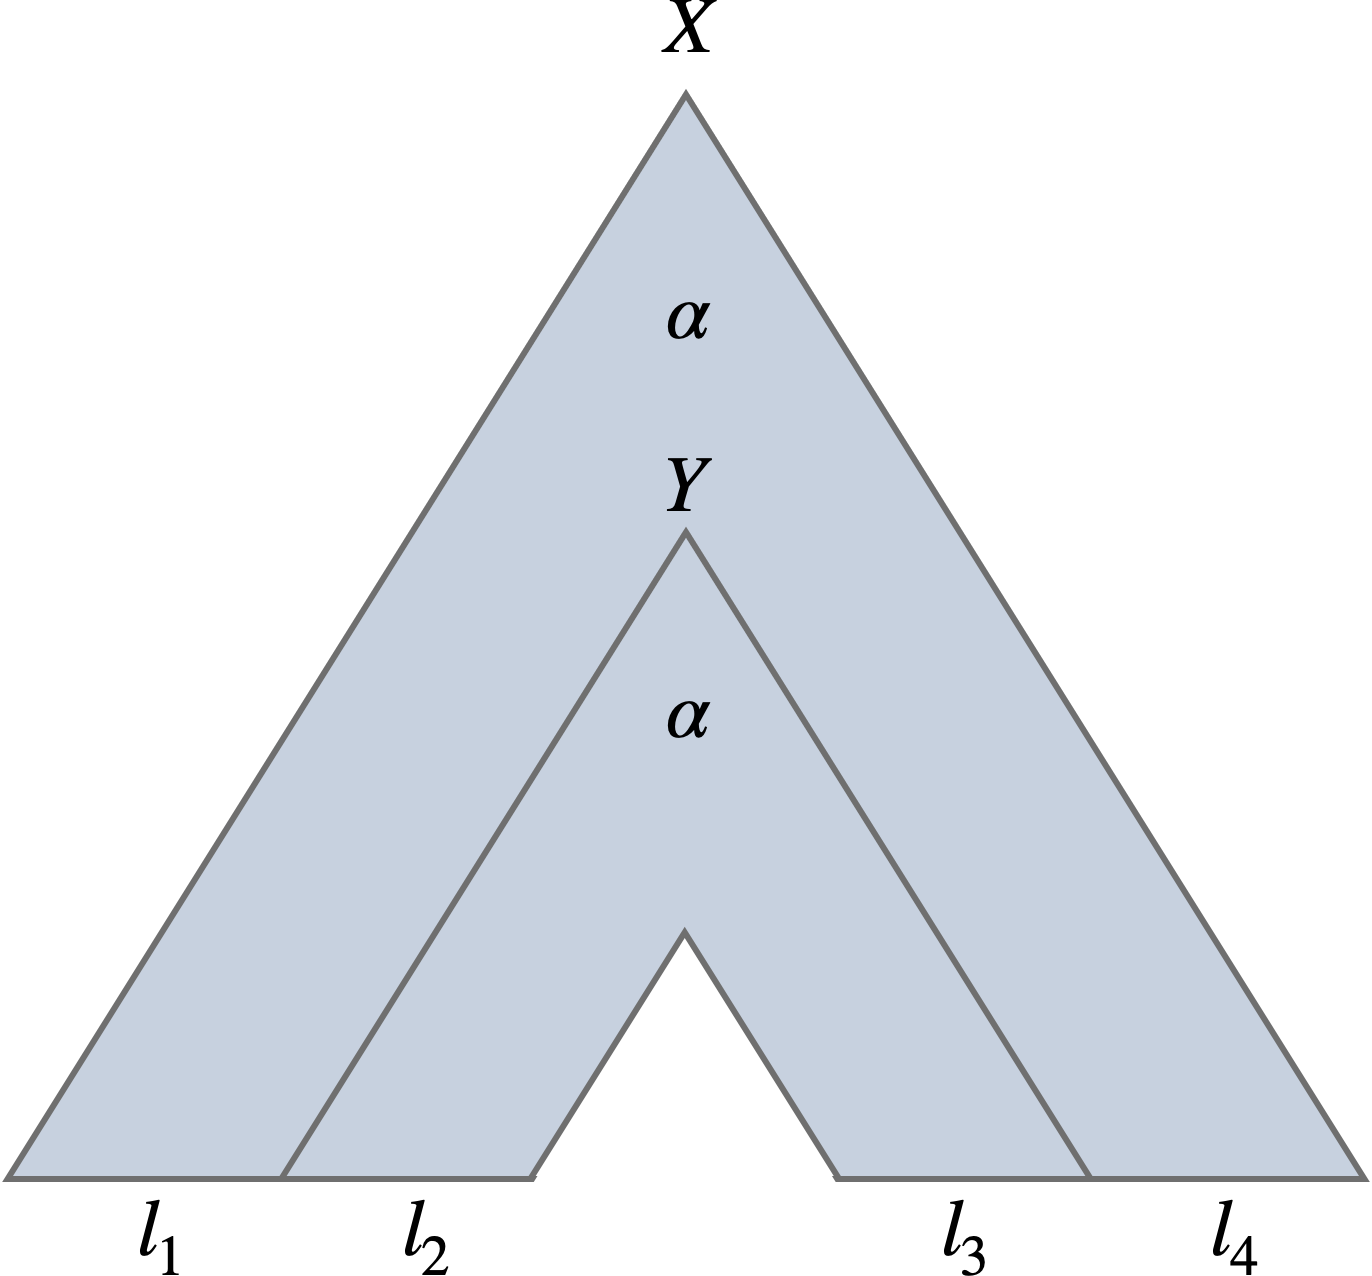
\includegraphics[width=\linewidth]{images/parsing/complete[Star][1].png}}
            \end{minipage} &
            \AxiomC{$X \xrightarrow{\alpha} [l_1,l_4]$}
            \AxiomC{$Y \xrightarrow{\beta} [l_2,l_3]$}
            \RightLabel{$\substack {X \overset{\alpha}{\leadsto} [Y]}$}
            \BinaryInfC{$X \xrightarrow {(\alpha,\langle \_\rangle, [\beta])} {[l_1+l_2,l_3+l_4]}$}
            \DisplayProof
        \end{tabular}
        
       
    

        \subsection{Proof of correctness}
    \section{Approximate parsing for Template grammar}
        \subsection{Tree compression}
        \subsection{A-star parsing}


    

\cleardoublepage
\part{Computational Experiments}
\chapter{Pattern discovery in Jazz Harmony Tree Bank}
    \section{Quantitative results and discussion}
    \section{Qualitative analysis}
\chapter{The plausibility of minimal-sized Template as Jazz harmonic analysis}
    \section{Many-to-one mapping from Template to CFG parse tree}
    \section{Baselines}
        \subsection{PCFG}
        \subsection{PACFG}
    \section{Quantitative results and discussion}
    \section{Qualitative analysis}
\chapter{Inducing Template grammar from Jazz chord progressions}
    \section{Method 1: Non-parametric Bayesian inference}
        \subsection{Pitman-Yor process prior}
    \section{Method 2: A heuristic based on tree compression} 
        \subsection{Straight-line tree grammar}
    \section{Comparison between the two methods}
   
\chapter{Contributions and conclusions}

% use to end the last part if the thesis is composed of parts
\addtocontents{toc}{\vspace{\normalbaselineskip}}
\cleardoublepage
\bookmarksetup{startatroot}

%%%%%%%%%%%%%%%%%%%%%%%%%%%%%%%%%%%%%%%%%%%%%%
%%%%% TAIL: Bibliography, Appendix, CV
%%%%%%%%%%%%%%%%%%%%%%%%%%%%%%%%%%%%%%%%%%%%%%
% \include{tail/appendix}
% \backmatter
% \include{tail/biblio}
% % Add your glossary here
% % Add your index here
% % Photographic credits (list of pictures&images that have been used with names of the person holding the copyright for them)
% \include{tail/cv}

\end{document}
